\documentclass[11pt]{report}
\usepackage[margin=2cm]{geometry}
\usepackage{graphicx}
\usepackage{float}
\usepackage{times}

\newcommand{\et}{et al.~} 
\usepackage{hyperref}

\usepackage[dvipsnames]{xcolor}

\newcommand{\Gap}{\texorpdfstring{\hfill}{}}
\newcommand{\Rec}{\texorpdfstring{{\small\emph{\color{blue}{\fbox{High Leverage}}}}}{}}
\newcommand{\HighRisk}{\texorpdfstring{{\small\emph{\color{orange}{\fbox{Uncertain Impact}}}}}{}}
\newcommand{\Longterm}{\texorpdfstring{{\small\emph{\color{OliveGreen}{\fbox{Long-term}}}}}{}}

\begin{document}

\section{Transportation\texorpdfstring{\hfill\textit{by Lynn H.~Kaack}}{}}
\label{sec:transportation}

Transportation systems form a complex web that is fundamental to an active and prosperous society. Globally, the transportation sector accounts for about a quarter of energy-related CO$_2$ emissions \cite{ipcc_global_2018}. 
In contrast to the electricity sector, however, transportation has not made significant progress to lower its CO$_2$ emissions \cite{Creutzig911} and much of the sector is regarded as hard to decarbonize \cite{Daviseaas9793}. This is because of the high energy density of fuels required for many types of vehicles, which constrains low-carbon alternatives, and because transport policies directly impact end-users and are thus more likely to be controversial.

Passenger and freight transportation are each responsible for about half of transport GHG emissions \cite{AR5_transport}. 
Both freight and passengers can travel by road, by rail, by water, or by air (referred to as \emph{transport modes}). Different modes carry vastly different carbon emission intensities.\footnote{Carbon intensity is measured in grams of CO$_2$-equivalent per person-km or per ton-km, respectively.}
At present, more than two-thirds of transportation emissions are from road travel \cite{AR5_transport}, but air travel has the highest emission intensity and is responsible for an increasingly large share.
Strategies to reduce GHG emissions\footnote{For general resources on how to decarbonize the transportation sector, see the AR5 chapter on transportation \cite{AR5_transport}, and \cite{figueroa2014energy, iea2017future, kaack2018decarbonizing}.} from transportation include \cite{AR5_transport}: 
\begin{itemize}
    \item Reducing transport activity.
    \item Improving vehicle efficiency.
    \item Alternative fuels and electrification.
    \item Modal shift (shifting to lower-carbon options, like rail).
\end{itemize}

\begin{figure}[tb]
    \centering
    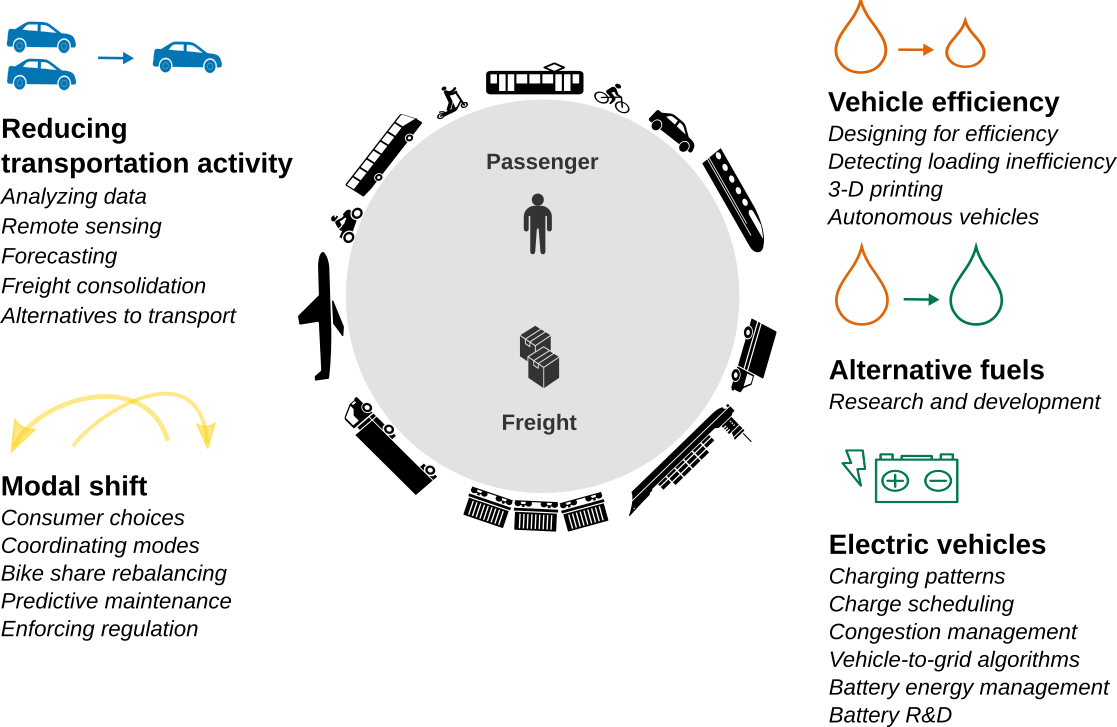
\includegraphics[width=\textwidth]{figures/transport.png}
    \caption{Selected strategies to mitigate GHG emissions from transportation using machine learning.}
    \label{fig:transport}
\end{figure}
Each of these mitigation strategies offers opportunities for ML (Fig.~\ref{fig:transport}).  
While many of us probably think of autonomous vehicles and ride-sharing when we think of transport and ML, these technologies have uncertain impacts on GHG emissions \cite{WADUD20161}, potentially even increasing them. 
We discuss these disruptive technologies in \S\ref{sec:TReducing} but show that ML can play a role for decarbonizing transportation that goes much further. 
ML can improve vehicle engineering, enable intelligent infrastructure, and provide policy-relevant information. 
Many interventions that reduce GHG emissions in the transportation sector require changes in planning, maintenance, and operations of transportation systems, even though the GHG reduction potential of those measures might not be immediately apparent. ML can help in implementing such interventions, for example by providing better demand forecasts. Typically, ML strategies are most effective in tandem with strong public policies.  
While we do not cover all ML applications in the transportation sector, we aim to include those areas that can conceivably reduce GHG emissions. 

\subsection{Reducing transport activity}\label{sec:TReducing}


A colossal amount of transport occurs each day across the world, but much of this mileage occurs inefficiently, resulting in needless GHG emissions. With the help of ML, the number of vehicle-miles traveled can be reduced by making long trips less necessary, increasing loading, and optimizing vehicle routing. Here, we discuss the first two in depth -- for a discussion of ML and routing, see for example \cite{ZENG2017458}. 

\paragraph*{Understanding transportation data}\mbox{}\\\label{sec:transport-data}Many areas of transportation lack data, and decision-makers often design infrastructure and policy with uncertain information. In recent years, new types of sensors have become available, and ML can turn this raw data into useful information.
Traditionally, traffic is monitored with ground-based counters that are installed on selected roads. A variety of technologies are used, such as inductive loop detectors or pneumatic tubes. Traffic is sometimes monitored with video systems, in particular when counting pedestrians and cyclists, which can be automated with computer vision \cite{Zaki2016361}.
Since counts on most roads are often available only over short time frames, these roads are modeled by looking at known traffic patterns for similar roads. ML methods, such as SVMs and neural networks, have made it easier to classify roads with similar traffic patterns \cite{krile2016assessing, tsapakis2015use, gastaldi2013annual}. 
As ground-based counters require costly installation and maintenance, many countries do not have such systems. Vehicles can also be detected in high-resolution satellite images with high accuracy \cite{sommer2017fast, jiang2015deep, mundhenk2016large, deng2017toward}, and image counts can serve to estimate average vehicle traffic \cite{kaack2019truck}. 
Similarly, ML methods can help with imputing missing data for precise bottom-up estimation of GHG emissions \cite{NOCERA2018125} and they are also applied in simulation models of vehicle emissions \cite{doi:10.1080/15568318.2017.1346732}. 


\paragraph*{Modeling demand}\Gap\textbf{\Rec}\mbox{}\\Modeling demand and planning new infrastructure can significantly shape how long trips are and which transport modes are chosen by passengers and shippers -- for example, discouraging sprawl and creating new transportation links can both reduce GHG emissions. 
ML can provide information about mobility patterns, which is directly necessary for agent-based travel demand models, one of the main transport planning tools \cite{feygin7932990}.
For example, ML makes it possible to estimate origin-destination demand from traffic counts \cite{MA201896}, and it offers new methods for spatio-temporal road traffic forecasting -- which do not always outperform other statistical methods \cite{doi:10.1080/01441647.2018.1442887} 
but may transfer well between areas \cite{Tang2018spatial}.
Also, short-term forecasting of public transit ridership can improve with ML; see for example \cite{Dai:2018aa, NOURSALEHI2018277}. 
ML is particularly relevant for deducing information from novel data -- for example, learning about the behavior of public transit users from smart card data \cite{Manley2018, Ghaemi_2017}.
Also, mobile phone sensors provide new means to understand personal travel demand and the urban topology, such as walking route choices \cite{doi:10.1177/0265813516659286}. 
Similarly, ML-based modeling of demand can help mitigate climate change by improving operational efficiency of modes that emit significant CO$_2$, such as aviation. ML can help predict runway demand and aircraft taxi time in order to reduce the excess fuel burned in the air and on the ground due to congestion in airports \cite{JACQUILLAT2018168, lee2015taxi}.



\paragraph*{Shared mobility}\Gap\textbf{\HighRisk}\mbox{}\\In the passenger sector, shared mobility (such as on-demand ride services or vehicle-sharing\footnote{In this section, we discuss shared cars; see \S\ref{sec:modalshift} for bike shares and electric scooters.}), is undoubtedly disrupting the way people travel and think about vehicle ownership, and ML plays an integral part in optimizing these services (e.g.~\cite{8317908}). 
However, it is largely unclear what the impact of this development will be. For example, shared cars can actually cause more people to travel by car, as opposed to using public transportation. Similarly, on-demand taxi services add mileage when traveling without a customer, possibly negating any GHG emission savings \cite{suatmadi2019demand}. 
On the other hand, shared mobility can lead to higher utilization of each vehicle, which means a more efficient use of materials \cite{Hertwich_2019}. The use of newer and more efficient vehicles, ideally electric ones, could increase with vehicle-sharing concepts, reducing GHG emissions. Some of the issues raised above could also perhaps be overcome by making taxis autonomous. Such vehicles also might integrate better with public transportation, and offer new concepts for pooled rides, which substantially reduce the emissions per person-mile.

ML methods can help to understand the energy impact of shared mobility concepts.
For example, they can be used to predict if a customer decides to share a ride with other passengers from an on-demand ride service \cite{CHEN201751}. For decision-makers it is important to have access to timely location-specific empirical analysis to understand if a ride share service is taking away customers from low-carbon transit modes and increasing the use of cars. Some local governments are beginning to require data-sharing from these providers (see \S\ref{sec:data_pol}).

Car-sharing services using autonomous vehicles could yield GHG emission savings when they encourage people to use public transit for part of the journey \cite{2017-01-1276} or with autonomous electric vehicles \cite{kang2016autonous}. However, using autonomous shared vehicles alone could increase the total vehicle-miles traveled and therefore do not necessarily lead to lower emissions as long as the vehicles have internal combustion engines (or electrical engines on a ``dirty'' electrical grid) \cite{lu2018multiagent, CHEN2016243}.
We see the intersection of shared mobility, autonomous and electric vehicles, and smart public transit as a path where ML can make a contribution to shaping future mobility. See also \S\ref{sec:TEfficient} for more on autonomous vehicles.

When designing and promoting new mobility services, it is important that industry and public policy prioritize lowering GHG emissions. Misaligned incentives in the early stages of technological development could result in the lock-in to a service with high GHG emissions \cite{AXSEN20191, 10.2307/2234208}.



\paragraph*{Freight routing and consolidation}\Gap\textbf{\Rec}\mbox{}\\Bundling shipments together, which is referred to as freight consolidation, dramatically reduces the number of trips (and therefore the GHG emissions). The same is true for changing routing so that trucks do not have to return empty. As rail and water modes require much larger loads than trucks, consolidation also enables shipments to use these modes for part of the journey \cite{kaack2018decarbonizing}. Freight consolidation and routing decisions are often taken by third-party \emph{logistics service providers} and other freight forwarders, such as in the less-than-truckload market, which deals with shipments of smaller sizes. ML offers opportunities to optimize this complex interaction of shipment sizes, modes, origin-destination pairs, and service requirements. Many problem settings are addressed with methods from the field of operations research. There is evidence that ML can improve upon these methods, in particular mixed-integer linear programming \cite{2018arXiv181106128B}. Other proposed and deployed applications of ML include predicting arrival times or demand, identifying and planning around transportation disruptions \cite{DHL}, and clustering suppliers by their geographical location and common shipping destinations. Proposed planning approaches include designing allocation algorithms and freight auctions, and ML has for example been shown to help pick good algorithms and parameters to solve auction markets \cite{Sandholm_very-large-scalegeneralized}. 



\paragraph*{Alternatives to transport}\Gap\textbf{\HighRisk}\mbox{}\\Disruptive technologies that are based on ML could replace or reduce transportation demand. 
For example, additive manufacturing (AM, or 3-D printing) has (limited) potential to reduce freight transport by producing lighter goods and enabling production closer to the consumer \cite{kaack2018decarbonizing}. ML can be a valuable tool for improving AM processes \cite{PhysRevLett.120.145301}. ML can also help to improve virtual communication \cite{Shiarlis}. If passenger trips are replaced by telepresence, travel demand can be reduced, as has been shown for example in public agencies \cite{ARNFALK2016101} and for scientific teams \cite{Marlow4841}. However, it is uncertain to what extent virtual meetings replace physical travel, or if they may actually give rise to more face-to-face meetings \cite{doi:10.1080/17450101.2014.902655}.

\subsection{Improving vehicle efficiency}\label{sec:TEfficient}
Most vehicles are not very efficient compared to what is technically possible: for example, aircraft carbon intensity is expected to decline by more than a third with respect to 2012, simply by virtue of newer models replacing aging jets \cite{schaefer2015}. Both the design of the vehicle and the way it is operated can increase the fuel economy. Here, we discuss how ML can help design more efficient vehicles and the impacts that autonomous driving may have on GHG emissions. Encouraging drivers to adopt more efficient vehicles is also a priority; while we do not focus on this here, ML plays a role in studying consumer preferences in vehicle markets \cite{burnap2016improving}.

\paragraph*{Designing for efficiency}\Gap\mbox{}\\There are many ways to reduce the energy a vehicle uses -- such as more efficient engines, improved aerodynamics, hybrid electric engines, and reducing the vehicle's weight or tire resistance.
These different strategies require a broad range of engineering techniques, many of which can benefit from ML. For example, ML is applied in advanced combustion engine design \cite{JANAKIRAMAN2016304}.
Hybrid electric vehicles, which are more efficient than combustion engines alone, rely on power management methods that can be improved with ML \cite{en11030476}. Aerodynamic efficiency improvements need turbulence modeling that is often computationally intensive and relies heavily on ML-based surrogate models \cite{YONDO201823}. Aerodynamic improvements can not only be made by vehicle design but also by rearranging load. Lai \et\cite{doi:10.1243/09544097JRRT92} use computer vision to detect aerodynamically inefficient loading on freight trains.  
Additive manufacturing (3-D printing) can produce lighter parts in vehicles, such as road vehicles and aircraft, that reduce energy consumption \cite{kaack2018decarbonizing, Hertwich_2019}. ML is applied to improve those processes, for example through failure detection \cite{Scime2018114, Shevchik2018598} or material design \cite{Gu2018939}. 

\paragraph*{Autonomous vehicles}\Gap\textbf{\HighRisk}\mbox{}\\Machine learning is essential in the development of autonomous vehicles (AVs), including in such basic tasks as following the road and detecting obstacles \cite{DBLP:journals/corr/BojarskiTDFFGJM16}.\footnote{Providing details on the general role of ML for AVs is beyond the scope of this paper.} While AVs could reduce energy consumption -- for example, by reducing traffic congestion and inducing efficiency through eco-driving -- it is also possible that AVs will lead to an increase in overall road traffic that nullifies efficiency gains. (For an overview of possible energy impacts of AVs see \cite{WADUD20161, Brown2014} and for broader impacts on mobility see \cite{Hancock7684}.)  Two advantages of AVs in the freight sector promise to cut GHG emissions: 
First, small autonomous vehicles, such as delivery robots and drones, could reduce the energy consumption of last-mile delivery \cite{samaras2018drones}, though they come with regulatory challenges \cite{marks2019law}. Second, trucks can reduce energy consumption by \emph{platooning} (driving very close together to reduce air resistance), thereby alleviating some of the challenges that come with electrifying long-distance road freight \cite{Guttenberg_2017}. Platooning relies on autonomous driving and communication technologies that allow vehicles to brake and accelerate simultaneously.

ML can help to develop AV technologies specifically aimed at reducing energy consumption. For example, Wu \et\cite{Wu2017EmergentBI,wu2017flow} develop AV controllers based on reinforcement learning to smooth out traffic involving non-autonomous vehicles, reducing congestion-related energy consumption. ML methods can also help to understand driving practices that are more energy efficient. For example, Jim\'enez et al.~\cite{en11020412} use data from smart phone sensors to identify driving behavior that leads to higher energy consumption in electric vehicles.

\subsection{Alternative fuels and electrification}\label{sec:TFuels}

\paragraph*{Electric vehicles}\Gap\textbf{\Rec}\mbox{}\\\label{sec:transport-evs}Electric vehicle (EV) technologies -- using batteries, hydrogen fuel cells, or electrified roads and railways -- are regarded as a primary means to decarbonize transport. EVs can have very low GHG emissions -- depending, of course, on the carbon intensity of the electricity. ML is vital for a range of different problems related to EVs. Rigas et al.~\cite{7000557} detail methods by which ML can improve charge scheduling, congestion management, and vehicle-to-grid algorithms. ML methods have also been applied to battery energy management (for example charge estimation \cite{HANSEN2005351} or optimization in hybrid EVs \cite{en11030476}), and to detect faults and lateral misalignment in wireless charging of EVs \cite{8096493}. 

As more people drive EVs, understanding their use patterns will become more important. Modeling charging behavior will be useful for grid operators looking to predict electric load. For this application, it is possible to analyze residential EV charging behavior from aggregate electricity load (\emph{energy disaggregation}, see also \S\ref{sec:use}) \cite{WANG20192611}. Also, in-vehicle sensors and communication data are increasingly becoming available and offer an opportunity to understand travel and charging behavior of EV owners, which can for example inform the placement of charging stations \cite{TAO2018735}. 

Battery electric vehicles are typically not used for more than a fraction of the day, allowing them to act as energy storage for the grid 
at other times, where charging and discharging is controlled for example by price signals \cite{doi:10.1002/wene.56} (see \S\ref{sec:electricity-variable},\ref{sec:electricity-currentSystemImpact}). There is much potential for ML to improve such vehicle-to-grid technology, for example with reinforcement learning \cite{VAZQUEZCANTELI20191072}, which can reduce GHG emissions from electricity generation. Vehicle-to-grid technology comes with private and social financial benefits. However, consumers are expected to be reluctant to agree to such services, as they might not want to compromise their driving range \cite{HIDRUE201567}. 

Finally, ML can also play a role in the research and development of batteries, a decisive technology for EV costs and usability. 
Work in this area has focused on predicting battery state, degradation, and remaining lifetime using supervised learning techniques, fuzzy logic, and clustering \cite{wu2016review, waag2014critical, si2011remaining, severson2019data, ellis2018new, hu2016advanced, kauwe2019data, buteau2019}.
However, many models developed in academia are based on laboratory data that do not account for real-world factors such as environmental conditions \cite{wu2016review, waag2014critical, si2011remaining}. By contrast, industry lags behind in ML modeling, but real-world operational data are readily available. Merging these two perspectives could yield significant benefits for the field.

\paragraph*{Alternative fuels}\Gap \textbf{\Longterm}\mbox{}\\Much of the transportation sector is highly dependent on liquid fossil fuels. Aviation, long-distance road transportation, and ocean shipping require fuels with high energy density and thus are not conducive to electrification \cite{Daviseaas9793}. Electrofuels \cite{BRYNOLF20181887}, solar fuels \ref{sec:electricity-materials}, biofuels \cite{biofuelsIEA}, hydrogen \cite{doeHydrogen, cano2018fuelCells}, and perhaps natural gas \cite{tong2015gas} offer alternatives, but the use of these fuels is constrained by factors such as cost, land-use, and (for hydrogen and natural gas) incompatibility with current infrastructure \cite{Daviseaas9793}.  
Electrofuels and biofuels have the potential to serve as low-carbon drop-in fuels that retain the properties of fossil fuels, such as high energy density, while retaining compatibility with the existing fleet of vehicles and the current fuel infrastructure \cite{kaack2018decarbonizing}. 
Fuels such as electrofuels and hydrogen can be produced using electricity-intensive processes and can be stored at lower cost than electricity. Thus, as a form of energy storage, these fuels could provide services to the electricity grid by enabling flexible power use and balancing variable electricity generators (\S\ref{sec:electricity-variable}). Given their relative long-term importance and early stage of development, they present a critical opportunity to mitigate climate change.
ML techniques may present opportunities for improvement at various stages of research and development of alternative fuels (similar to applications in  \S\ref{sec:electricity-variable}). 


\subsection{Modal shift}\label{sec:modalshift}
Shifting passengers and freight to low carbon-intensity modes is one of the most important means to decarbonize transport. 
This \emph{modal shift} in passenger transportation can for example involve providing people with public transit, which requires analyzing mode choice and travel demand data. ML can also make low-carbon freight modes more competitive by helping to coordinate intermodal transport.

\paragraph*{Passenger preferences }\Gap\mbox{}\\ML can improve our understanding about passengers' travel mode choices, which in turn informs transportation planning, such as where public transit should be built. 
Some recent studies have shown that supervised ML based on survey data can improve passenger mode choice models \cite{omrani2015predicting, nam2017model, HAGENAUER2017273}. 
Seo \et propose to conduct long-term travel surveys with online learning, which reduces the demand on respondents, while obtaining high data quality \cite{SEO2017}. 
Sun \et \cite{SUN201896} use SVMs and neural networks for analyzing preferences of customers traveling by high speed rail in China. 
There is also work on inferring people's travel modes and destinations from social media or various mobile phone sensors such as GPS (\emph{transportation mode detection}), e.g.~\cite{DABIRI2018360, doi:10.1080/13658816.2017.1356464}.  Also in the freight sector, ML has been applied to analyze modal trade-offs, for example by imputing data on counterfactual mode choices \cite{doi:10.1080/03081060.2011.600092}.

\paragraph*{Enabling low-carbon options}\Gap\textbf{\Rec}\label{sec:LCcompetitive}\mbox{}\\In order to incentivize more users to choose low-carbon transport modes, their costs and service quality can be improved.
Many low-carbon modes must be integrated with other modes of transportation to deliver the same level of service. For example, when traveling by train, the trip to and from the station will often be by car, taxi, bus, or bike. There are many opportunities for ML to facilitate a better integration of modes, both in the passenger and freight sectors.
ML can also help to improve the operation of 
low-carbon modes, for example by reducing the operations and maintenance costs of rail \cite{JAMSHIDI2018185} and predicting track degradation \cite{doi:10.1177/0954409716657849}. 

Bike sharing and electric scooter services can offer low-carbon alternatives for urban mobility that do not require ownership and integrate well with public transportation. ML studies help to understand how usage patterns for bike stations depend on their immediate urban surroundings \cite{HYLAND201871}.
ML can also help solve the bike sharing rebalancing problem, where shared bikes accumulate in one location and are lacking in other locations, by improving forecasts of bike demand and inventory \cite{REGUE2014192}. Singla \et  \cite{Singla:2015:IUB:2887007.2887108} propose a pricing mechanism based on online learning to provide monetary incentives for bike users to help rebalancing. By producing accurate travel time estimates, ML can provide tools that help to integrate bike shares with other modes of transportation \cite{8005582}.
Many emerging bike and scooter sharing services are dockless, which means that they are parked anywhere in public space and can block sidewalks \cite{anderson2019governing}. ML has been applied to monitor public sentiment about such bike shares via tweets \cite{doi:10.1177/0361198119838982}. ML could also provide tools and information for regulators to ensure that public space can be used by everyone \cite{citylab2019race}. 

Coordination between modes resulting in faster and more reliable transit times could increase the amount of people or goods traveling on low-carbon modes such as rail. 
ML algorithms could be applied to make public transportation faster and easier to use. For example, there is a rich literature exploring ML methods to predict bus arrival times and their uncertainty \cite{altinkaya2013bus, MAZLOUMI2011534}.
Often freight is packaged so that it can switch between different modes of transport easily. Such \emph{intermodal} transportation relies on low-carbon modes such as rail and water for part of the journey \cite{kaack2018decarbonizing}.
ML can contribute by improving predictions of the estimated time of arrival (for example of freight trains \cite{BARBOUR2018211}) or the weight or volume of expected freight (for example for roll-on/roll-off transport -- often abbreviated as Ro-Ro \cite{doi:10.1111/itor.12337}). Intelligent transport systems of different modes could be combined and enable more efficient multimodal freight transportation \cite{kaack2018decarbonizing}.


Some modes with high GHG emissions, such as trucks, can be particularly cost-competitive in regions with lax enforcement of regulation, as they can benefit from overloading and not obeying labor or safety rules \cite{kaack2018decarbonizing}. 
ML can assist public institutions with enforcing their regulations. For example, image recognition can help law enforcement detect overloading of trucks \cite{2018AIPC.1955d0038Z}.

\subsection{Discussion}
Decarbonizing transport is essential to a low-carbon society, and there are numerous applications where ML can make an impact. This is because transportation causes a large share of GHG emissions, but reducing them has been slow and complex. Solutions are likely very technical, are highly dependent on existing infrastructure, and require detailed understanding of passengers' and freight companies' behavior. ML can help decarbonize transportation by providing data, gaining knowledge from data, planning, and automation. Moreover, ML is fundamental to shared mobility, AVs, EVs, and smart public transit, which, with the right incentives, can be used to enable significant reductions in GHG emissions.

\end{document}
